\documentclass[sigconf]{acmart}

\AtBeginDocument{ \providecommand\BibTeX{ Bib\TeX } }
\setcopyright{acmlicensed}
\copyrightyear{2025}
\acmYear{2025}
\acmDOI{XXXXXXX.XXXXXXX}

\acmConference[BI 2025]{Business Intelligence}{-}{-}

\begin{document}

\title{BI2025 Experiment Report - Group 088}
%% ---Authors: Dynamically added ---

          \author{Maria Salmasian}
          \authornote{Student A, Matr.Nr.: 12537811}
          \affiliation{
            \institution{TU Wien}
            \country{Austria}
          }
          
          \author{Brais Guardado Collazo}
          \authornote{Student B, Matr.Nr.: 12233000}
          \affiliation{
            \institution{TU Wien}
            \country{Austria}
          }
          

\begin{abstract}
  This report documents the machine learning experiment for Group 088, following the CRISP-DM process model.
\end{abstract}

\ccsdesc[500]{Computing methodologies~Machine learning}
\keywords{CRISP-DM, Provenance, Knowledge Graph, Machine Learning}

\maketitle

%% --- 1. Business Understanding ---
\section{Business Understanding}

\subsection{Data Source and Scenario}
The data source is the Dry Bean Dataset, manually collected by the department of computer engineering of the Selcuk University, Turkey. It contains 13611 instances of 7 different dry bean varieties processed into 16 different morphological features (e.g. area, perimeter, major axis length...) via computer vision.

According to the literature, dry beans are the most important and most produced pulses over the world. Assessment of the best seed is the main problem for dry bean producers and markets. Traditionally, bean classification is performed manually, which is a difficult process as well as very time consuming and inefficient at scale. Misclassification errors can also occur, which lead to quality inconsistencies and customer rejections.

\subsection{Business Objectives}
Two main business objectives can be identified: to automate the dry bean classification problem, cutting operational costs and to minimize misclassification errors induced by this sorting process.

\subsection{Business Success Criteria}
Some business success criteria tied to the objectives:
- Reduce customer returns by 5\%.
- Cut labor costs by 30\%.
- 50\% increase in sorting speed.

\subsection{Data Mining Goals}
We propose the following goals:
- Training of two multiclass classification models.
- If model supports it, quantify feature importance and explainability.

\subsection{Data Mining Success Criteria}
- Trained classifier achieves >95\% accuracy.
- Identification of the 5 most important features for classification.

\subsection{AI Risk Aspects}
We deem the task of dry bean classification relatively harmless in terms of possible AI Risks identified by the EU AI Act. However, some considerations must be noted:

- Data bias and generalization: the dataset originates from a controlled set of images. Trained models may rely on specific lighting conditions or zoom/scale, failing when faced with real world production environments
- ML Security: computer vision backed models are susceptible to be targeted by adversarial attacks. In this context, a successful attack (intentional or not) could trigger a misclassification, contaminating the batch.

%% --- 2. Data Understanding ---
\section{Data Understanding}
\textbf{Dataset Description:} Morphological features describing seven dry bean classes.

The following features were identified in the dataset:

\begin{table}[h]
  \caption{Raw Data Features}
  \label{tab:features}
  \begin{tabular}{lp{0.2\linewidth}p{0.4\linewidth}}
    \toprule
    \textbf{Feature Name} & \textbf{Data Type} & \textbf{Description} \\
    \midrule
    Area & integer> & The area of a bean zone and the number of pixels within its boundaries. \\
    Aspect ratio & double> & Defines the relationship between the major and minor axis lengths. \\
    Class & string> & The bean variety \\
    Compactness & double> & Measures the roundness of an object \\
    Convex area & integer> & Number of pixels in the smallest convex polygon that can contain the area of a bean seed. \\
    Eccentricity & double> & Eccentricity of the ellipse having the same moments as the region. \\
    Equivalent diameter & double> & The diameter of a circle having the same area as a bean seed area. \\
    Extent & double> & The ratio of the pixels in the bounding box to the bean area. \\
    Major axis length & double> & The distance between the ends of the longest line that can be drawn from a bean. \\
    Minor axis length & double> & The distance of the longest line that can be drawn from the bean while standing perpendicular to the main axis. \\
    Perimeter & double> & Bean circumference is defined as the length of its border. \\
    Roundness & double> & Ratio of area over the squared of the perimeter \\
    Solidity & double> & The ratio of the pixels in the convex shell to those found in beans. \\
    \bottomrule
  \end{tabular}
\end{table}

\subsection{Outlier Analysis}
A z-score based method (threshold = 2.2) was used to identify extreme values in numeric attributes. This step was exploratory and did not directly determine which data instances should be removed.

After inspecting the boxplots, one extreme instance was identified in the ShapeFactor4 attribute for the Seker class. This instance was considered an outlier and removed, while all other data points were kept.

\subsection{Statistical Properties}
The dataset contains 13611 records and 16 numeric attributes. Attribute 'Area' has mean=53048.28, std=29324.10, min=20420.00, max=254616.00. Attribute 'Perimeter' has mean=855.28, std=214.29, min=524.74, max=1985.37. Attribute 'MajorAxisLength' has mean=320.14, std=85.69, min=183.60, max=738.86. Attribute 'MinorAxisLength' has mean=202.27, std=44.97, min=122.51, max=460.20. Attribute 'AspectRation' has mean=1.58, std=0.25, min=1.02, max=2.43. Attribute 'Eccentricity' has mean=0.75, std=0.09, min=0.22, max=0.91. Attribute 'ConvexArea' has mean=53768.20, std=29774.92, min=20684.00, max=263261.00. Attribute 'EquivDiameter' has mean=253.06, std=59.18, min=161.24, max=569.37. Attribute 'Extent' has mean=0.75, std=0.05, min=0.56, max=0.87. Attribute 'Solidity' has mean=0.99, std=0.00, min=0.92, max=0.99. Attribute 'roundness' has mean=0.87, std=0.06, min=0.49, max=0.99. Attribute 'Compactness' has mean=0.80, std=0.06, min=0.64, max=0.99. Attribute 'ShapeFactor1' has mean=0.01, std=0.00, min=0.00, max=0.01. Attribute 'ShapeFactor2' has mean=0.00, std=0.00, min=0.00, max=0.00. Attribute 'ShapeFactor3' has mean=0.64, std=0.10, min=0.41, max=0.97. Attribute 'ShapeFactor4' has mean=1.00, std=0.00, min=0.95, max=1.00. Strong correlations for attribute pairs: Area and Perimeter (r=0.97); Area and MajorAxisLength (r=0.93); Area and MinorAxisLength (r=0.95); Area and ConvexArea (r=1.00); Area and EquivDiameter (r=0.98); Area and ShapeFactor1 (r=-0.85); Perimeter and MajorAxisLength (r=0.98); Perimeter and MinorAxisLength (r=0.91); Perimeter and ConvexArea (r=0.97); Perimeter and EquivDiameter (r=0.99); Perimeter and ShapeFactor1 (r=-0.86); Perimeter and ShapeFactor2 (r=-0.77); MajorAxisLength and MinorAxisLength (r=0.83); MajorAxisLength and ConvexArea (r=0.93); MajorAxisLength and EquivDiameter (r=0.96); MajorAxisLength and ShapeFactor1 (r=-0.77); MajorAxisLength and ShapeFactor2 (r=-0.86); MinorAxisLength and ConvexArea (r=0.95); MinorAxisLength and EquivDiameter (r=0.95); MinorAxisLength and ShapeFactor1 (r=-0.95); AspectRation and Eccentricity (r=0.92); AspectRation and roundness (r=-0.77); AspectRation and Compactness (r=-0.99); AspectRation and ShapeFactor2 (r=-0.84); AspectRation and ShapeFactor3 (r=-0.98); Eccentricity and roundness (r=-0.72); Eccentricity and Compactness (r=-0.97); Eccentricity and ShapeFactor2 (r=-0.86); Eccentricity and ShapeFactor3 (r=-0.98); ConvexArea and EquivDiameter (r=0.99); ConvexArea and ShapeFactor1 (r=-0.85); EquivDiameter and ShapeFactor1 (r=-0.89); EquivDiameter and ShapeFactor2 (r=-0.71); Solidity and ShapeFactor4 (r=0.70); roundness and Compactness (r=0.77); roundness and ShapeFactor2 (r=0.78); roundness and ShapeFactor3 (r=0.76); Compactness and ShapeFactor2 (r=0.87); Compactness and ShapeFactor3 (r=1.00); ShapeFactor2 and ShapeFactor3 (r=0.87).

\subsection{Data Quality Assessment}
No missing values were detected in the dataset. Attribute 'Area' shows a strongly skewed distribution (skewness=2.95), indicating an uneven distribution of values. Attribute 'Perimeter' shows a strongly skewed distribution (skewness=1.63), indicating an uneven distribution of values. Attribute 'MajorAxisLength' shows a strongly skewed distribution (skewness=1.36), indicating an uneven distribution of values. Attribute 'MinorAxisLength' shows a strongly skewed distribution (skewness=2.24), indicating an uneven distribution of values. Attribute 'Eccentricity' shows a strongly skewed distribution (skewness=-1.06), indicating an uneven distribution of values. Attribute 'ConvexArea' shows a strongly skewed distribution (skewness=2.94), indicating an uneven distribution of values. Attribute 'EquivDiameter' shows a strongly skewed distribution (skewness=1.95), indicating an uneven distribution of values. Attribute 'Solidity' shows a strongly skewed distribution (skewness=-2.55), indicating an uneven distribution of values. Attribute 'ShapeFactor4' shows a strongly skewed distribution (skewness=-2.76), indicating an uneven distribution of values. 7106 records were identified as potential outliers using the existing z-score based outlier detection method (threshold = 2.2). Outliers were detected in the following attributes: Area, Perimeter, MajorAxisLength, MinorAxisLength, AspectRation, Eccentricity, ConvexArea, EquivDiameter, Extent, Solidity, roundness, Compactness, ShapeFactor1, ShapeFactor2, ShapeFactor3, ShapeFactor4. These extreme values may represent rare but valid cases and should be handled carefully to avoid reducing the representation of uncommon patterns.

\subsection{Visual Data Exploration}
\begin{figure}
    \centering
    \includegraphics[width=1\linewidth]{img/plot_heatmap.png}
    \caption{Correlation between features}
    \label{fig:feature_corr}
\end{figure}
% Comment

\begin{figure}
    \centering
    \includegraphics[width=1\linewidth]{img/plot_histogram.png}
    \caption{Histogram for the Area feature}
    \label{fig:area_histogram}
\end{figure}
% Comment

The distribution of attribute 'Area' was visually inspected using a histogram, revealing its spread and central tendency. The distribution of attribute 'Perimeter' was visually inspected using a histogram, revealing its spread and central tendency. The distribution of attribute 'MajorAxisLength' was visually inspected using a histogram, revealing its spread and central tendency. The distribution of attribute 'MinorAxisLength' was visually inspected using a histogram, revealing its spread and central tendency. A correlation heatmap was generated to visually assess relationships between numeric attributes, supporting hypotheses about linear dependencies. Based on the visual exploration, it is hypothesized that size-related attributes exhibit strong positive relationships, while shape-related attributes vary more independently.

\begin{figure}
    \centering
    \includegraphics[width=1\linewidth]{img/plot_boxplot.png}
    \caption{Boxplot for ShapeFactor4 for all classes}
    \label{fig:shpft4_boxplot}
\end{figure}

From the Figure \ref{fig:shpft4_boxplot} we can clearly identify an outlier. There is a data instance belonging to the Seker dry bean class which lies extremely far away from the other values of ShapeFactor4 in this class.


\subsection{Ethical and AI Risk Aspects}
Ethical sensitivity, minority groups, and distributional bias: The dataset has numeric geometric and morphological attributes that come from object measurements.  No attributes have personal, demographic, socio-economic, or identifiable information. So the dataset does not contain ethically sensitive attributes.  However, strongly skewed distributions for several attributes indicate not well represented regions of the feature space, showing rare or extreme geometric configurations. These may lead to representation bias in modeling tasks, where common patterns dominate model behavior.  Potential risks, bias sources, and expert questions: There are some potential risks. Strong skewness and extreme values show representation bias against uncommon shapes and sizes. Strong correlations among size-related attributes show possible sampling bias toward objects on similar scale. The lack of detailed data provenance questions data acquisition, selection criteria, and prior preprocessing steps. To better assess bias and data quality risks, these questions may help: Does the dataset reflect real-world variability of object shapes and sizes? Were certain object types or ranges excluded during collection? Are extreme values rare in reality or under-represented due to sampling or preprocessing decisions?  Required data preparation actions: Data preparation should handle skewed attributes, preserve rare cases, manage correlated features, and use evaluation metrics that account for imbalance. Improving data provenance would increase transparency.

%% --- 3. Data Preparation ---
\section{Data Preparation}
\subsection{Data Cleaning}
Removed all instances of the SEKER class where `ShapeFactor4` was below 0.95.

We have considered scaling some of the features with highest mean, like the area or the perimeter. However, we consider this scaling (done or not) cannot be performed before train/validation/test splitting due to possible data leakage. Test set instances should never influence how much the train and validation sets are scaled.

Adding more derived attributes does not seem truly necessary, as many of the already exisiting features are already derivations of other measures. So much so, that the four last attributes are simply called "ShapeFactorX".

Additional information that could be interesting to add into the dataset is some form of color information. According to the original paper where this dataset is presented, all dry bean images were first converted into black and white images for feature extraction. At the same time, we know that one of the dry bean varieties, the Barbunya, possesses certain colourful characteristics, that are lost during b/w conversion.


%% --- 4. Modeling ---
\section{Modeling}

\subsection{Hyperparameter Configuration}
The model was trained using the following hyperparameter settings:

\begin{table}[h]
  \caption{Hyperparameter Settings}
  \label{tab:hyperparams}
  \begin{tabular}{lp{0.4\linewidth}l}
    \toprule
    \textbf{Parameter} & \textbf{Description} & \textbf{Value} \\
    \midrule
    C & Regularization parameter (controls margin vs misclassification). & 50 \\
    n\_estimators & Number of trees in the forest & 50 \\
    \bottomrule
  \end{tabular}
\end{table}

\subsection{Training Run}
A training run was executed with the following characteristics:
\begin{itemize}
    \item \textbf{Algorithm:} Support Vector Classifier (SVC) Algorithm
    \item \textbf{Start Time:} 2026-01-14 14:37:44
    \item \textbf{End Time:} 2026-01-14 14:37:49
    \item \textbf{Result:}  = 
\end{itemize}

%% --- 5. Evaluation ---
\section{Evaluation}
A dummy classifier has been chosen as baseline. Such a classifier makes predictions without taking into account any of the features, but rather predicts based on simple rules. For our case, we chose to "train" this dummy classifier to always predict the most numerous class. This yielded a macro accuracy of just 26.01\%.

The reported best performing model by the literature achieves a macro accuracy of 93.13\%, obtained by a SVM model. The Bombay dry bean class was perfectly classified in that scenario. On the other hand, the most difficult variety to classify was the Sira class, achieving only an 86.84\% accuracy.

\begin{figure}
    \centering
    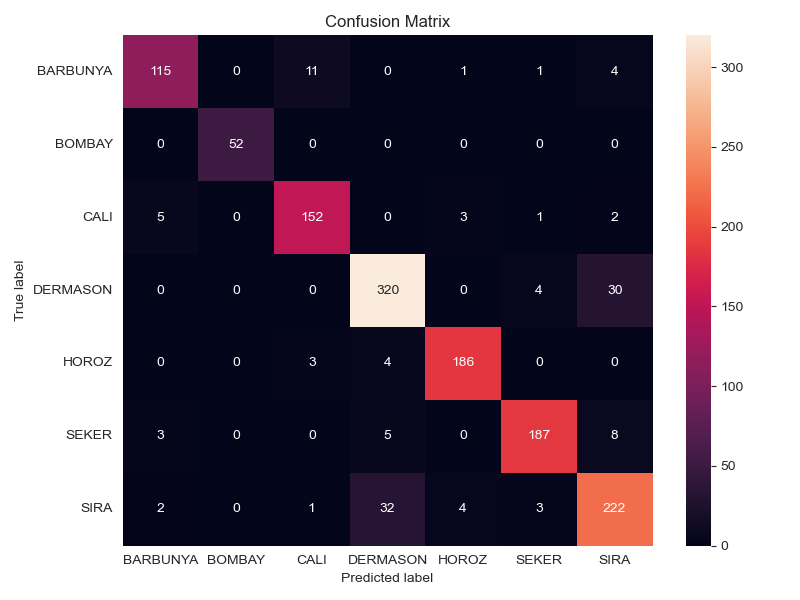
\includegraphics[width=1\linewidth]{confusion_matrix.png}
    \caption{Final RF performance on the test set}
    \label{fig:rf-conf-matrix}
\end{figure}

\begin{figure}
    \centering
    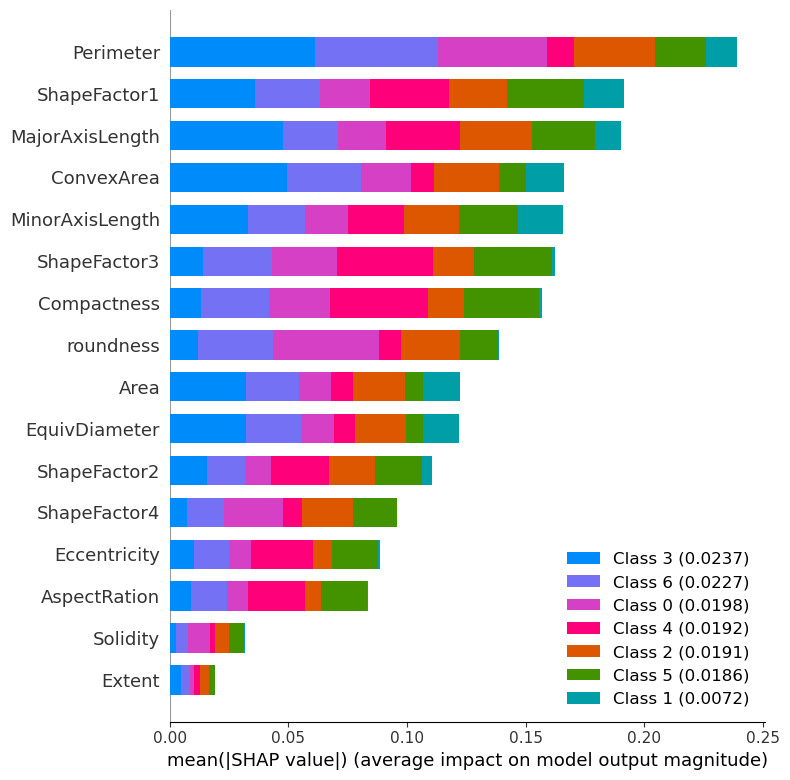
\includegraphics[width=1\linewidth]{shapley_values.png}
    \caption{Feature importance analysis via SHAP values}
    \label{fig:shapley-values}
\end{figure}

Our final model (random forest classifier) achieves an overall macro accuracy of 91.18\% and 92.6\% F1 score. Most notably, the Bombay class has also been perfectly identified, while we obtain an 84.09\% accuracy on the Sira class, as we can see in Figure \ref{fig:rf-conf-matrix}.

Regarding feature importance, we performed SHAP value analysis for a small subset (first 100 rows) of the test set. The results can be seen in Figure \ref{fig:shapley-values}. According to it, we identify the top 5 most important features as follows: Perimeter, ShapeFactor1, MajorAxisLength, ConvexArea, MinorAxisLength.

Regarding the success criteria defined in the Business Understanding phase, we can say that we do not fulfill them all. We set out to achieve at least 95\% accuracy, failing short by just 4 points. The second success criteria is successfully met, as we have identified not only the top 5, but all feature importances using Shapley values.

In principle, there seems to be no "protected attribute". In fact, the identification of such an attribute in a black box model such as a RF with more than a hundred trees is not really feasible. But, we can indeed identify three features which, as a whole, could undeniably identify one class. Those are the area, minor axis length and shape factor 1; which could be used to identify the Bombay class with high accuracy (both in the literature and in our work, 100\% accuracy is obtained on this class).

%% --- 6. Deployment ---
\section{Deployment}
\subsection{Business Objectives Reflection and Deployment Recommendations}
The trained models on this project have not been deployed in any real world scenario, since this would go way beyond the scope of the assignment. The business objectives defined in the first phase serve as a reference for what could be interesting insights for stakeholders. Without a proper deployment, it is difficult to assess whether the new system would indeed reduce customer returns or labor costs. Increasing the sorting speed is most likely limited by hardware, not by the classification model itself.
\subsection{Ethical Aspects and Risks}
The dataset contains only numeric geometric and morphological measurements and does not include personal, demographic, or sensitive attributes. So, no direct ethical risks related to privacy or discrimination or  high-risk AI aspects were identified. However, skewed feature distributions and class imbalance may lead to representation bias, where rare classes or extreme patterns are predicted less accurately. This risk was identified during data understanding and should be considered when interpreting model outputs in deployment.
\subsection{Monitoring Plan}
Once deployed, monitor the model's performance using metrics like macro F1 and per-class recall. It is advised to pay special attention to minority classes, as their results may decline over time. If macro F1 decreases or recall for any class becomes very low, conduct further analysis and consider retraining the model.
\subsection{Reproducibility Reflection}
All steps in the whole data mining pipeline presented in this notebook have been properly documented using PROV-O and other relevant ontologies, hopefully creating a rich provenance graph. Moreover, all function calls which require a random initialization have been provided with a fixed random seed (42). Other aspects which could negatively affect reproducibility, such as hardware or software versions used, have not been documented. A conda YAML file is provided, but it does not enforce exact package versions. All code above is also dependent on a customly written (and still in development) Python package to interact with an external RDF triplestore. Though unlikely, breaking changes cannot be ruled out.

\section{Conclusion}

\end{document}
